\documentclass{beamer}

\usepackage{graphicx}
\usepackage{hyperref}
\usepackage[latin1]{inputenc}
\usepackage[T1]{fontenc}
\usepackage[english]{babel}
\usepackage{listings}
\usepackage{xcolor,mathrsfs,url}
\usepackage{amssymb}
\usepackage{amsmath}
\usepackage{ifthen}

\usepackage{metricsbeamer} % using the metric beamer style

% The command to define a subsection is '\subsec{}' and NOT '\subsection'.
% This code generates the bar. Don't edit.
\newcommand{\midbarnew}{}
\newcommand{\subsec}[1]
{
  \ifthenelse{\equal{#1}{}}
  {\renewcommand{\midbarnew}{} \subsection{}}
  {\renewcommand{\midbarnew}{ $\mid$ } \subsection{#1}}
}

% change the pictures here, if necessary. logobig and logosmall are the internal names
% for the pictures: do not modify them, just change "hulogo" and "logo". Pictures must be 
% supplied as JPEG, PNG or PDF
%########################################

\pgfdeclareimage[height=2cm]{logobig}{hulogo} % use hucase instead for the Humboldt-Case Logo
\pgfdeclareimage[height=1cm]{logosmall}{hulogo}

% use this number to modify the scaling of the headline on titlepage
\def\titlescale{1.0}


\def\authora{Your Name}	% First Author
\def\affa{Humboldt-Universit�t zu Berlin, Institute for Statistics and Econometrics} % First Author's Affiliation
\def\authorb{Her Name}  % Second Author
\def\affb{Humboldt-Universit�t zu Berlin} % Second Author's Affiliation
\def\authorc{His Name}  % Third Author
\def\affc{Humboldt-Universit�t zu Berlin} % Third Author's Affiliation

\def\linka{}	% Link to your institution's/ personal website
\def\linkb{}
\def\linkc{}
\def\email{\href{mailto:your.email@address.com}{your.email@address.com}}	% Your email address

\title[Short Title]{The title of the talk can even be much \\ longer than this}
\institute{Institute for Statistics and Econometrics \\ Chair of Econometrics \\ Humboldt-Universit�t zu Berlin}

%Start of the document
\begin{document}
\Section{}

\frame[plain]{% create the titleslide, layout controlled in metricsbeamer
	\titlepage
}

\Section{Introduction}

\frame{% how to print
\frametitle{How to print\dots}
\begin{center}
\begin{figure}
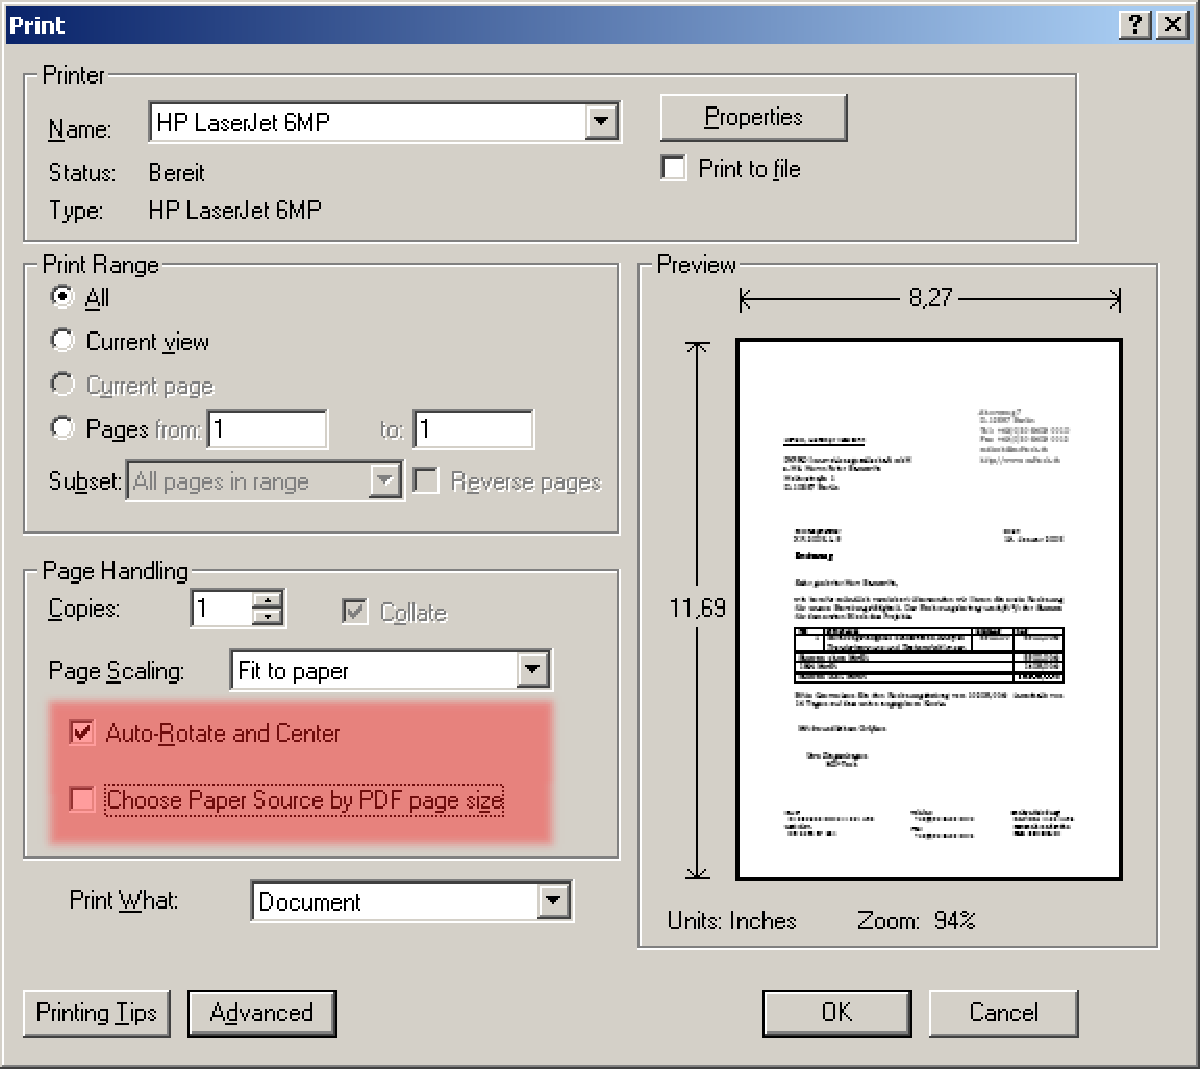
\includegraphics[width=0.5\textwidth]{howtoprint.pdf}
\caption{Hallo}
\end{figure}
\end{center}
}

\frame{
\frametitle{Basics}
Statistics is understanding data by modeling it.

Data \( Y^{(n)} = (Y_{1},\ldots,Y_{n}) \) usually \emph{random}.

\( I\!\!P = \mathscr{L}(Y^{(n)}) \), the \emph{unknown} joint distribution.

Statistical problem: to infer on \( I\!\!P \) from the data \( Y^{(n)} \).

\emph{Parametric} modeling:
\begin{eqnarray*}
I\!\!P = I\!\!P_{\boldsymbol{\theta}} \in (I\!\!P_{\boldsymbol{\theta}}, \boldsymbol{\theta} \in \Theta \subset I\!\!R^{p}).
\end{eqnarray*}

\emph{Nonparametric} modeling:
the parametric assumption is not fulfilled, or, equivalently,
}

\frame{
\frametitle{Outline}

\begin{enumerate}
\item \alert{attract the audience}
\item the scientific message
\item explain the method
\item simulations \& discussion of your results
\item applications and examples
\item almost EOT = end of talk
\item provoke few questions
\item audience: enjoy what you have learnt
\end{enumerate}


}

\frame{
\frametitle{Math Environments}

\begin{definition}
Definition environment
\end{definition}

\begin{theorem}
Theorem environment
\end{theorem}

\begin{example}
Example environment
\end{example}

}

\Section{Section}
\subsec{Optional: Subsection} % The command to define a subsection is '\subsec{}' and NOT '\subsection'.

\frame{
\frametitle{The title of the slide}

\begin{itemize}
\item \texttt{Beamer} is the latest package to create slides with \LaTeX
	\begin{itemize}
		\item Nested: Level 2
		\item Nested: Level 2
			\begin{itemize}
				\item Nested: Level 3
			\end{itemize}
	\end{itemize}
\item slides need to be compiled to PDF, not DVI/Postscript
\item Remember: PDFLaTeX accepts PNG, JPEG and PDF not EPS/PS
\item some adjustments for ISE were made, so use Section instead of section
\end{itemize}
}

\frame{
	\frametitle{Making Tables}
	\begin{table}
		\begin{tabular}{lccc}
		\hline\hline
		Column 1 & Column 2 & Column 3 & Column 4 \\
		\hline
		Some	& Numbers	& 1			& 2		\\
		3		& 4			& 5			& 6		\\
		\hline
		\hline
		\end{tabular} 
		\caption{A sample table}  
	\end{table}
	
} 


\beamertemplatebookbibitems
\frame{
\frametitle{For Further Reading}
\begin{thebibliography}{aaaaaaaaaaaaaaaaa}
\bibitem[H�rdle, 2003]{haerdle2003}
W.~H�rdle and L.~Simar
\newblock {\em Applied Multivariate Statistical Analysis}
\newblock Springer, 2003
\beamertemplatearticlebibitems
\bibitem[Dijkstra, 1982]{Dijkstra1982}
E.~Dijkstra.
\newblock Smoothsort, an alternative for sorting in situ.
\newblock {\em Science of Computer Programming}, 1(3):223--233, 1982.
\beamertemplatebookbibitems
\bibitem{eckel}
Frank Mittelbach and Michel Goossens
\newblock {\em The \LaTeX{ }Companion -- 2nd ed.}
\newblock Addison-Wesley, 2004
\end{thebibliography}
}


\end{document}

